%%%%%%%%%%%%%%%%%%%%%%%%%%%%%%%%%%%%%%%%%%%%%%%%%%%%%%%%%%%%%%%
%
% Welcome to Overleaf --- just edit your article on the left,
% and we'll compile it for you on the right. If you give
% someone the link to this page, they can edit at the same
% time. See the help menu above for more info. Enjoy!
%
%%%%%%%%%%%%%%%%%%%%%%%%%%%%%%%%%%%%%%%%%%%%%%%%%%%%%%%%%%%%%%%
%
% For more detailed article preparation guidelines, please see:
% http://f1000research.com/author-guidelines

\documentclass[10pt,a4paper,twocolumn]{article}
\usepackage{f1000_styles}
\usepackage{url}
\usepackage{listings}

%% Default: numerical citations
% \usepackage[numbers]{natbib}

%% Uncomment this lines for superscript citations instead
% \usepackage[super]{natbib}

%% Uncomment these lines for author-year citations instead
\usepackage[round]{natbib}
\let\cite\citep

\begin{document}

\title{iSEE: Interactive SummarizedExperiment Explorer}
\author[1,$\dagger$]{Kevin Rue-Albrecht}
\author[2,3,$\dagger$]{Federico Marini}
\author[4,$\dagger$]{Charlotte Soneson}
\author[5,$\dagger$,$\ast$]{Aaron T. L. Lun}

\affil[1]{Kennedy Institute of Rheumatology, University of Oxford, Oxford OX3 7FY, United Kingdom}
\affil[2]{Center for Thrombosis and Hemostasis (CTH), University Medical Center of the Johannes Gutenberg University Mainz, Mainz}
\affil[3]{Institute for Medical Biostatistics, Epidemiology and Informatics (IMBEI), University Medical Center of the Johannes Gutenberg University Mainz, Mainz}
\affil[4]{University of Zurich and SIB Swiss Institute of Bioinformatics, Zurich, Switzerland}
\affil[5]{Cancer Research UK Cambridge Institute, University of Cambridge, Cambridge CB2 0RE, United Kingdom}
\affil[$\dagger$]{These authors contributed equally.}
\affil[$\ast$]{To whom correspondence should be addressed.}


\maketitle
\thispagestyle{fancy}

% Please list all authors that played a significant role in the research involved in the article. Please provide full affiliation information (including full institutional address, ZIP code and e-mail address) for all authors, and identify who is/are the corresponding author(s).
% TODO: full address and emails too? if so, in which format do we provide them?

\begin{abstract}
Data exploration is critical to the comprehension of large biological data sets generated by high-throughput assays such as sequencing.
However, most existing tools for interactive visualization are limited to specific assays or analyses.
Here, we present the iSEE (Interactive SummarizedExperiment Explorer) software package, which provides a general visual interface for exploring data in a SummarizedExperiment object.
iSEE is directly compatible with many existing R/Bioconductor packages for analyzing high-throughput biological data,
and provides useful features such as simultaneous examination of multiple data aspects, dynamic linking between plots and code tracking for reproducibility.
We demonstrate the utility and flexibility of iSEE by applying it to explore a range of real transcriptomics and proteomics data sets.

% Abstracts should be up to 300 words and provide a succinct summary of the article. Although the abstract should explain why the article might be interesting, care should be taken not to inappropriately over-emphasize the importance of the work described in the article. Citations should not be used in the abstract, and the use of abbreviations should be minimized. If you are writing a Research or Systematic Review article, please structure your abstract into Background, Methods, Results, and Conclusions.

\end{abstract}

\section*{Keywords}

% Please list up to eight keywords to help readers interested in your article find it more easily.

Single-cell, gene expression, transcriptomics, proteomics, visualization, interactive, shiny, Bioconductor

% TODO: refine keywords

\clearpage

\section*{Introduction}
Interactive data exploration is critical to the analysis and comprehension of the data generated by high-throughput biological assays such as genomics.
Exploration drives the formation of novel data-driven hypotheses prior to a more rigorous statistical analysis, and enables diagnosis of potential problems such as batch effects and low-quality samples.
To this end, visualization of the data in an intuitive and interactive interface is crucial, allowing researchers to examine the data from different perspectives across samples (e.g., experimental replicates, patients, single cells) and features (e.g., genes, transcripts, proteins, genomic regions).\\

Most existing tools for interactive visualization of biological data are designed for specific assays and analyses, e.g., pRoloc for proteomics \citep{gatto2014mass}, shinyMethyl for methylation \citep{fortin2014shinymethyl}, HTSvis for high-throughput screens \citep{scheeder2017htsvis}.
Opportunities for customization are generally limited, making it difficult to re-use the same visualization software for new technologies or experimental designs where different aspects of the data are of interest.
Moreover, standalone tools such as the Loupe Cell Browser from 10X Genomics \citep{zheng2017massively} do not easily integrate into established analysis pipelines such as those based on the R statistical programming language \citep{rcore2008R}.
This complicates any coordinated use of these tools with a reproducible, transparent, and statistically rigorous analysis.\\

Here, we present the iSEE software package for interactive data exploration.
iSEE is implemented in R using the Shiny framework \citep{chang2017shiny} and exploits data structures from the open-source Bioconductor project \citep{gentleman2004bioconductor}, specifically the SummarizedExperiment class.
iSEE allows users to simultaneously visualize multiple aspects of a given data set, including experimental data, metadata and analysis results.
Dynamic linking and point selection facilitate the flexible exploration of interactions between different data aspects.
Additional functionalities include code tracking, intelligent downsampling of large data sets, custom colour scale specification and tour construction.
We demonstrate the capabilities of iSEE by applying it to a diverse range of real data sets.

\section*{Taking a SummarizedExperiment input}
The iSEE interface is initialized with a single function call accepting a SummarizedExperiment object as input \citep{huber2015orchestrating}.
Each instance of the SummarizedExperiment class stores one or more matrices of experimental observations as ``assays'', where rows and columns represent genomic features and biological samples, respectively.
For instance, individual assays may represent gene expression matrices of raw counts along with different normalization strategies.
In addition, per-feature or per-sample variables are stored in the ``rowData'' and ``colData'', respectively; those may include experimental metadata as well as any analysis results.\\

The flexibility of the SummarizedExperiment class is the driving factor behind its broad deployment throughout the Bioconductor ecosystem.
SummarizedExperiment objects are currently used in analysis pipelines for RNA sequencing \citep{love2014moderated}, methylation \citep{aryee2014minfi} and Hi-C data \citep{lun2016infrastructure}, amongst others.
Package developers can also easily use the base SummarizedExperiment class to derive new bespoke classes for particular applications, such as the SingleCellExperiment class for single-cell 'omics data.
By accepting SummarizedExperiment objects as input, iSEE immediately offers interactive visualization for a variety of data modalities.
This complements the state-of-the-art analysis workflows and methodologies already available in R/Bioconductor packages. \\

\section*{Interface implementation}

\subsection*{Using a multi-panel layout}
All data aspects stored in a SummarizedExperiment can be readily examined alongside one another in the multi-panel layout of the iSEE interface (Fig.~\ref{fig:iSEE}A).
The interface layout is built using the shinydashboard package \citep{chang2018shinydashboard}, using colour-coded panels to visualize each data aspect.
Individual panel types include:

\begin{itemize}
\item Column data plots, for visualizing sample metadata stored in the colData slot of SummarizedExperiment object.
\item Feature expression plots, for visualizing expression values for a particular feature (e.g., gene) across samples from any assay in the SummarizedExperiment object.
Despite its name, this plot type is applicable to data modalities beyond gene expression.
\item Row statistics tables, to present the contents of the rowData slot for the SummarizedExperiment object.
\item Row data plots, for visualizing sample metadata stored in the rowData slot of a SummarizedExperiment object.
\item Heat maps, to visualize assay data for multiple features where samples are ordered by one or more colData fields.
\item Reduced dimension plots, which display any two dimensions from pre-computed dimensionality reduction results (e.g., from PCA or $t$-SNE).
These results are taken from the reducedDim slot of any SingleCellExperiment object supplied to iSEE.
\end{itemize}

\begin{figure*}[t]
\includegraphics[width=\textwidth]{pics/Fig1.pdf}
\caption{iSEE uses a customisable multi-panel layout (A) that simultaneously displays one or more panels of various types, where each panel type visualizes a different aspect of the data.
New panels of any type can be added (i), and all panels can be removed, reordered or resized (ii).
Panel types are available to visualize sample-based reduced dimensionality embeddings (iii), sample-level metadata (iv), and experimental observations across samples for each feature (v).
Other panel types include row statistics tables (vi), to facilitate searching across features and their metadata; heatmaps (vii), to visualize experimental observations for multiple features; and feature-level metadata plots.
Panels of each type are colour-coded for ease of interpretation.
(B) Information can be transmitted between panels according to a user-specified scheme.
Here, the selection of feature $X$ in the row statistics table determines the y-axis of the feature expression plot, and colours the samples in the reduced dimension plot by the expression of $X$.
Selection of points in the reduced dimension plot (dotted blue line) also determines the samples that are shown in the column data (i.e., sample metadata) plot;
further selection of points in the column data plot determines the samples that are shown in the heatmap.
}
\label{fig:iSEE}
\end{figure*}

Each sample is represented as a point in column data, feature expression and reduced dimension plots.
Similarly, each feature is represented by a point in row data plots.
For these panel types, a scatter plot is automatically produced if the selected variables on the x- and y-axes are both continuous.
If exactly one variable is categorical, points are grouped by the categorical levels and a (horizontal) violin plot is produced with points scattered within each violin.
If both variables are categorical, a ``rectangle plot'' is produced where each combination of categorical levels is represented by a rectangle with area proportional to the frequency of that combination.
Points are scattered randomly within each rectangle.
For ease of interpretation, the rectangle plot collapses to a mirrored bar plot when one of the categorical variables only has one level.

\subsection*{Custom panel colouring}
Sample-based points can be coloured according to the values of any sample-level metadata field in the colData or by the assay values of a selected feature.
Similarly, feature-based points can be coloured according to any feature-level metadata field in the rowData.
Heatmaps are coloured according to the expression values of the selected features in the chosen assay,
with additional colouring of each of the colData fields used to order the samples.
In all cases, the variable to use for colouring can be dynamically selected for each plot.
This enables users to easily examine relationships between different variables in a single plot. \\

By default, colour maps for categorical and continuous variables are taken from the ggplot2 \citep{wickham2009ggplot2} and viridis packages \citep{garnier2018viridis}, respectively.
However, iSEE also implements the ExperimentColorMap class, which allows users to specify arbitrary colour maps for particular variables.
Each colour map is a function that returns a vector of distinct colours of a specified length, and will be called whenever the associated variable is used for point colouring in a particular panel.
The returned colours will be mapped to factor levels for categorical variables, or used in colour interpolation for continuous variables.
For categorical variables, the function may also return a constant vector of named colors corresponding to the levels of a known factor.
Colour maps can be specified for individual variables; for all assays, all column data variables, or all row data variables (with different functions for continuous or categorical variables); or for all categorical or continuous variables.
This provides a convenient yet flexible mechanism for customization of colouring schemes within the interface.

\subsection*{Dynamic linking between panels}
A key feature of iSEE is the ability to dynamically transmit information between panels (Fig.~\ref{fig:iSEE}B).
Users can define and reorganize arbitrary links between ``transmitting'' and ``receiving'' panels, whereby selections in transmitting panels control the inclusion and appearance of the corresponding data points in receiving panels.
This feature facilitates exploration of the relationships between different aspects of the data.
For example, users can easily determine co-expression patterns of genes in a particular region of a reduced dimensionality embedding -- this is achieved by selecting points in a reduced dimension plot (using the standard rectangular brush or a lasso) and transmitting that selection to any number of feature expression plots.\\

This linking paradigm extends to multiple panels, whereby a panel can transmit to multiple receivers, and a receiving panel can transmit its own selection to another plot.
Chains of linked plots allow users to mimic the arbitrarily complex gating strategies often found in analyses of flow cytometry data \citep{finak2014opencyto}.
With iSEE, this concept is extended to any assay data, feature-level or sample-level metadata present in a SummarizedExperiment object, providing a powerful framework for interrogating multiple interactions between data aspects.
Row statistics tables can also transmit to various plot types, by selecting a table row to control the coloring of sample-based points;
or by defining a subset of features to visualize in a heatmap.
Furthermore, row data plots can transmit to row statistics tables, whereby selection of points in the former will subset the latter.

\subsection*{Code tracking and reproducibility}

iSEE automatically memorizes the exact R code that was used to generate every plot, extending previous work by \cite{marini2016interrepro}.
This code is fully accessible to users at any time during the run-time of the interface.
By integrating the code reported by iSEE into their own scripts, users can easily reproduce the results of any exploratory analysis.
Similarly, the code required to reproduce the current state of the interface can also be reported.
This can be used in startup scripts to launch an iSEE instance in any preferred layout, including the panel organization, variable selection, colouring schemes, links between panels and even individual brushes and lasso selections.

\subsection*{Additional functionalities}
Row statistics tables can be augmented with dynamic annotation based on the selected row, linking to online resources such as Ensembl or Entrez. % do we need to cite them? at least ENSEMBL has updated citable papers
For large data sets, points can be downsampled in a density-dependent manner to accelerate rendering of the plots, improving the responsiveness of the interface without compromising the fidelity of the visualization.
Users can also include a bespoke step-by-step ``tour'' of their data set via the rintrojs package \cite{ganz2016rintrojs}, guiding the audience through an examination of the salient features in the data.

\section*{Use cases} % FM: used often in other software articles in F1000res

\subsection*{Plate-based single-cell RNA sequencing}
To demonstrate iSEE's functionality, we used it to explore a plate-based single-cell RNA sequencing (scRNA-seq) data set involving 379 cells from the mouse visual cortex \citep{tasic2016allen}.
This demonstration guides the user through the main features of the iSEE interface including the multi-panel layout, colouring and dynamic linking.\\

Link: \url{http://shiny.imbei.uni-mainz.de:3838/iSEE/}

\subsection*{Droplet-based single-cell RNA sequencing}
We applied iSEE to a larger scRNA-seq data set involving 4,000 peripheral blood mononuclear cells (PBMCs), generated by 10X Genomics \citep{zheng2017massively}.
This demonstration explores the differences between different methods for distinguishing cells from empty droplets in droplet-based scRNA-seq protocols \citep{lun2018distinguishing}.\\

Link: \url{http://shiny.imbei.uni-mainz.de:3838/iSEE_PBMC4k/}

\subsection*{Bulk RNA sequencing from TCGA}
We applied iSEE to bulk RNA sequencing data from The Cancer Genome Atlas (TCGA) project, using a subset of expression profiles involving 7,706 tumor samples \citep{piccolo2015TCGA}.
This demonstration examines the elevation of \textit{HER2} expression in breast cancer samples.\\

Link: \url{http://shiny.imbei.uni-mainz.de:3838/iSEE_TCGA/}

\subsection*{Mass cytometry}
Finally, we explored a mass cytometry study involving 150,000 PBMCs from multiple donors before and after stimulation with BCR/FcR-XL \citep{bodenmiller2012cytof}.
We used iSEE to vizualise and refine a gating analysis to obtain B cells, and to investigate differences in expression of the functional marker pS6 after stimulation.\\

Link: \url{http://shiny.imbei.uni-mainz.de:3838/iSEE_cytof/}

\section*{Conclusion}
iSEE provides a general interactive interface for visual exploration of high-throughput biological data sets.
Any study that can be represented in a SummarizedExperiment object can be used as input, allowing iSEE to accommodate a diverse range of `-omics data sets.
The interface is flexible and can be dynamically customized by the user; supports exploration of interactions between data aspects through colouring and linking between panels;
and provides transparency and reproducibility during the interactive analysis, through code tracking and state reporting. 
The most obvious use of iSEE is that of data exploration for hypothesis generation during the course of a research project.
However, we also anticipate that public instances of iSEE will accompany publications to enable authors to showcase salient aspects of their work using guided tours.

\section*{Data and software availability}
The iSEE package is available at \url{https://bioconductor.org/packages/iSEE}.
Source code of the development version of the package is available at \url{https://github.com/csoneson/iSEE}.
Code for the demonstrations and tours is available at \url{https://github.com/LTLA/iSEE2018}.

\section*{Author contributions}
All authors contributed conceptually and technically to the development and maintenance of large sections of the package code.
ATLL and FM developed the application and data infrastructure.
KRA and CS developed the plotting framework.
FM developed the code tracking and user interface.
KRA designed and developed the ExperimentColorMap class.
All authors contributed to testing the application on all data sets.
All authors wrote and approved the final manuscript.

\section{Competing interests}
No competing interests were declared.

\section{Grant information}
ATLL was supported by core funding from Cancer Research UK (award no. 17197 to Dr.\ John Marioni).
The work of FM is supported by the German Federal Ministry of Education and Research (BMBF 01EO1003).

\section{Acknowledgements}
We thank the organizers and participants of the European Bioconductor Meeting 2017, where the idea for this package was first conceived.
We also thank members of the Bioconductor community for their helpful suggestions.

{\small\bibliographystyle{unsrtnat}
\bibliography{ref}}

\bigskip
% References can be listed in any standard referencing style that uses a numbering system
% (i.e. not Harvard referencing style), and should be consistent between references within
% a given article.

% For more author guidance please see:
% http://f1000research.com/author-guidelines


% When all authors are happy with the paper, use the
% ‘Submit to F1000Research' button from the menu above
% to submit directly to the open life science journal F1000Research.

% Please note that this template results in a draft pre-submission PDF document.
% Articles will be professionally typeset when accepted for publication.

% We hope you find the F1000Research Overleaf template useful,
% please let us know if you have any feedback using the help menu above.


\end{document}
